
\section{Finite Impulse Response (FIR) Filters}
FIR filters have an LCCDE and impulse response of the form
\begin{align*}
	y[n] = \sum\limits_{k=0}^{M-1} b_ku[n-k] &&\Rightarrow&& h = \{ b_0, b_1, \hdots, b_{M-1} \}
\end{align*}
and are therefore always stable. 

\subsubsection{Definitions}
\begin{center}
\renewcommand{\arraystretch}{1}
\renewcommand{\tabcolsep}{4pt}
\hspace*{-4pt}
\begin{tabular}{lll}
	$M$: filter length & $M-1$: filter order & $b_k$: filter coefficients
\end{tabular}
\end{center}\vspace*{-1em}

\subsubsection{Transfer Function and Frequency Response}
\vspace{-1em}
\begin{align*}
	H(z) = \sum\limits_{k=0}^{M-1} h[k] z^{-k} && H(\Omega) = \sum\limits_{k=0}^{M-1} \underbrace{h[k]}_{b_k} e^{-j\Omega k}
\end{align*}
\vspace{-1em}


\subsection{Moving Average (MA) Filter}
\subsubsection{LCCDE and Frequency Response}
The MA filter averages the current and past inputs to produce its output and is represented by the following LCCDE
\begin{align*}
	y[n] &= \frac{1}{M} \sum\limits_{k=0}^{M-1} u[n-k]
\end{align*}
Its frequency response is
\begin{align*}
	H(\Omega) &= \frac{1}{M}\sum\limits_{k=0}^{M-1}e^{-j\Omega k} = \frac{1}{M}\frac{1-e^{-j\Omega M}}{1-e^{-j\Omega}}
\end{align*}
Zeros therefore occur at $\Omega = 2\pi k / M$ where $k>0$ is an integer.

\subsubsection{Phase Response}
For small frequencies $\Omega$, the phase can be approximated by
\begin{align*}
	\angle H(\Omega) \approx -\frac{\Omega(M-1)}{2}
\end{align*}

\subsubsection{Magnitude Response}
The magnitude response of an MA filter is
\begin{align*}
	\abs{H(\Omega)} &= \frac{1}{M}\abs{\frac{\sin\!\left(\frac{\Omega M}{2}\right)}{\sin\!\left(\frac{\Omega}{2}\right)}} \xrightarrow{M\to\infty}\abs{\frac{\sin\!\left(\frac{\Omega M}{2}\right)}{\frac{\Omega M}{2}}} = \abs{\textrm{sinc}\!\left(\frac{\Omega M}{2}\right)}
\end{align*}

\subsection{Non-Causal Moving Average (NCMA) Filter}
The NCMA filter has the following impulse response
\begin{align*}
	h &= \{ \hdots, 0, \frac{1}{M}, \hdots, \underset{\uparrow}{\frac{1}{M}}, \hdots, \frac{1}{M}, 0, \hdots \}
\end{align*}
And the filter's frequency response is given by
\begin{align*}
	H(\Omega) &= \frac{1}{M}\sum\limits_{k=0}^{M-1}e^{-j\Omega\left(k-\frac{M-1}{2}\right)} = e^{j\Omega\left(\frac{M-1}{2}\right)}H_\text{MA}(\Omega)
\end{align*}
where $H_\text{MA}$ is the frequency response of the causal MA filter. Therefore, the frequency response of the NCMA filter has an added phase of $\Omega(M-1)/2$ compared to the MA filter. The magnitude, however, stays the same.

\subsection{Weighted Moving Average (WMA) Filter}
The WMA filter places less emphasis on older inputs
\begin{align*}
	y[n] = \frac{1}{S}\sum\limits_{k=0}^{M-1}w_ku[n-k] && S = \frac{M(M+1)}{2}
\end{align*}
$S$ is the normalization constant chosen such that the sum of all filter coefficients equals one. (often $w_k = (M-k)$)

\subsection{Non-Causal WMA (NCWMA) Filter}
The impulse response of an NCWMA filter is
\begin{align*}
	h[n] = \frac{1}{S}\tilde{h}[n] && S = \sum\limits_{k=-\infty}^\infty \tilde{h}[n]
\end{align*}
\vspace{-0.25em}
where $\tilde{h}[n]$ is given by
\vspace{-0.8em}
\begin{center}
	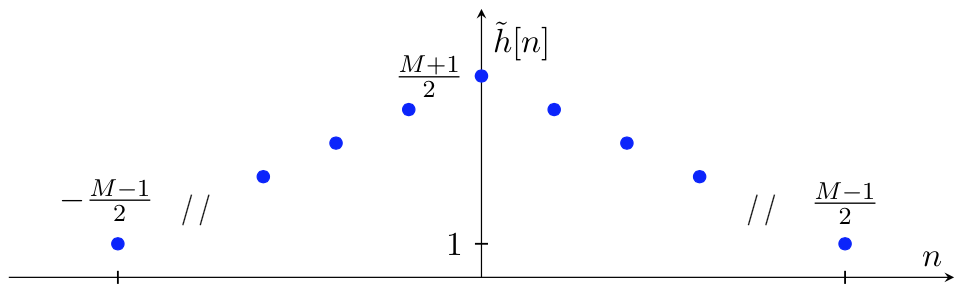
\includegraphics[width = .7\linewidth]{Filtering/NCWMAImpulseResponse.png}
\end{center}
An NCWMA Filter does \textbf{not} add any phase.\\
In general, if $H(z)$ is the transfer function of a MA filter with $M$ coefficients, then $H(z)H(z^{-1})$ is a non-causal WMA filter with $2M-1$ coefficients. 

